\documentclass[conference]{IEEEtran}
\IEEEoverridecommandlockouts
% The preceding line is only needed to identify funding in the first footnote. If that is unneeded, please comment it out.
\usepackage{cite}
\usepackage{amsmath,amssymb,amsfonts}
\usepackage{algorithmic}
\usepackage{graphicx}
\usepackage{textcomp}
\usepackage{xcolor}
\usepackage{hyperref}
\def\BibTeX{{\rm B\kern-.05em{\sc i\kern-.025em b}\kern-.08em
    T\kern-.1667em\lower.7ex\hbox{E}\kern-.125emX}}
\begin{document}

\title{Simulation of Personal Health Devices in WBAN networks\\
% {\footnotesize \textsuperscript{*}Note: Sub-titles are not captured in Xplore and
% should not be used}
% \thanks{Identify applicable funding agency here. If none, delete this.}
}

\author{\IEEEauthorblockN{1\textsuperscript{st} Given Name Surname}
\IEEEauthorblockA{\textit{dept. name of organization (of Aff.)} \\
\textit{name of organization (of Aff.)}\\
City, Country \\
email address}
\and
\IEEEauthorblockN{2\textsuperscript{nd} Given Name Surname}
\IEEEauthorblockA{\textit{dept. name of organization (of Aff.)} \\
\textit{name of organization (of Aff.)}\\
City, Country \\
email address}
\and
\IEEEauthorblockN{3\textsuperscript{rd} Given Name Surname}
\IEEEauthorblockA{\textit{dept. name of organization (of Aff.)} \\
\textit{name of organization (of Aff.)}\\
City, Country \\
email address}
\and
\IEEEauthorblockN{4\textsuperscript{th} Given Name Surname}
\IEEEauthorblockA{\textit{dept. name of organization (of Aff.)} \\
\textit{name of organization (of Aff.)}\\
City, Country \\
email address}
\and
\IEEEauthorblockN{5\textsuperscript{th} Given Name Surname}
\IEEEauthorblockA{\textit{dept. name of organization (of Aff.)} \\
\textit{name of organization (of Aff.)}\\
City, Country \\
email address}
\and
\IEEEauthorblockN{6\textsuperscript{th} Given Name Surname}
\IEEEauthorblockA{\textit{dept. name of organization (of Aff.)} \\
\textit{name of organization (of Aff.)}\\
City, Country \\
email address}
}

\maketitle

\begin{abstract}
% This document is a model and instructions for \LaTeX.
% This and the IEEEtran.cls file define the components of your paper [title, text, heads, etc.]. *CRITICAL: Do Not Use Symbols, Special Characters, Footnotes, 
% or Math in Paper Title or Abstract.
\end{abstract}

\begin{IEEEkeywords}
wban, personal health devices, antidote, castalia
\end{IEEEkeywords}

\section{Introduction}
\section{Related Works}\label{relatedworks}

Wireless sensor network have been employed and developed to support the research on specific and general-purpose WSN. 
% **colocar na introdução ** Due to the high cost to deploy a real WSN system, simulators is a low-cost option to test the realistic behavior before network before the real implementation.
With the popularization of the 11073 standard several improvements and researches have been made for the smooth operation, interoperability between the devices, and for the simulators of WBAN's.

In \cite{b6} the authors presents an open-source energy-harvesting simulation framework called GreenCastalia which supports multi-source and multi-storage energy harvesting architectures developed for the Castalia simulator. GreenCastalia project main focus is to simulate a realistic battery discharge on devices. The majors modifications to the original Castalia code was made to the Resource Manager module. Also in this module the authors adds the energy-harvesting systems that provides a more realistic battery model.

In \cite{b7},\cite{b8},\cite{b9} and \cite{b10} is proposed the integration of ISO/IEEE 11073 and the IOT protocols such as MQTT and COaP as transport protocols to enable the personal health devices directly shares health information through the Internet using low power consumption and few control messages. Also in those works is discussed the availability of enabling IOT technologies for the health information as well as the mapping of the messages from 11073 standard into the IOT protocols. Unlike the first work, these last four papers used real devices with Antidote as application layer protocol.

Another project on 11073 standards is \cite{b11} that has developed an interoperable  end-to-end remote patient monitoring platform using ZigBee Health Care Profile as transport layer and a Machine to Machine (M2M) solution to provide wide area network connectivity. This work also include a web application on the clinical side (server side) and use the stadandars and frameworks provided by Integrating the Healthcare Enterprise (IHE) \cite{b13} and Health Leven Seven (HL7) \cite{b12} to ensure end-to-end interoperability. These two companies advocate a world in which everyone can securely access and use the right health data when and where they need it.

A Point of Care version of the interoperability standard ISO/IEEE 11073 (X73-PoC) provide a mechanism to control remotely the agents. This mechanism is defined in the standards X73-10201 and X73-20301. However, the version of X73 oriented to Personal Health Devices has no mechanisms to do such a thing. So, in \cite{b14} the author proposes to adapt the remote control capabilities from X73-PoC to X73-PHD with an acceptable overhead and no extra cost to the manufacturers. This mechanism has to be installed in manager and in the agent. The remote control consists of being able to change units of measure from kilograms to pounds and vice versa directly from the manager, a smartphone or a compute engine
in nursing units.

\section{System Architecture}

Antidote has a plug-in based architecture. So, it was developed a Castalia plugin to support communication between Antidote Stack and Castalia Modules. As the Antidote Library was developed to work with real devices, modifications have been made to the library in reason to work in Castalia Simulator. Communication, encoders, agent and manager are some Antidote's modules changed.

\subsection{Castalia Plugin}

Antidote itself is portable and use ANSI C language to create a standard and clean library. But providing communication between Antidote and others systems, like Castalia, is plug-in dependent. So the dependence of Antidote is just in communication plug-ins.

The proposed plug-in allows Castalia and Antidote talks with each other through \textit{external variables}. Inside Castalia Simulator we can call any function from Antidote Library this way we can retrieve any information from Antidote library. The problem is to transmit the data from Castalia to Antidote Library. To solve this, we first use external variables to make the data exchange between Castalia and Castalia plug-in module. Then, to obtain the data from Castalia plug-in module, Antidote uses pointers to Plug-in Module functions. That's why we need a plug-in to mediate the communication. 

There are a set of callback functions in Castalia plug-in module that is passed to Antidote during the initialization process of agents. These callback functions are passed to communication module as pointers to functions.
This way whenever the communication module needs to retrieve or send a message it just trigger the correspondent callback function. The task of these callback functions is to receive and send messages as also initialize and finalize a agent network.

\subsection{Changes in communication module}

The Communication module is one of the most important modules in the Antidote. The start, the finalization, transmissions, machine state phases of all nodes are controlled by this module. In a real scenario, each device has your own communication module, running your own copy of the code. So, in one-machine simulation it is a bit different. Only one communication module has to handle with all nodes, since the Antidote Library is installed in the operating system as a dynamic library.

To ensure the proper functioning of communication module, the \textit{node id} is required in each method call, this way we know what node we are working with and apply the action just to that node, never affecting another node. For example, if a node transits from unassociated state to associating machine state, without the proposed modification, this action would affect all nodes even those who should not change their machine state.

The Fig.~\ref{fig:communicationModuleCastalia} illustrates the system modification.

\begin{figure}[htbp]
\centerline{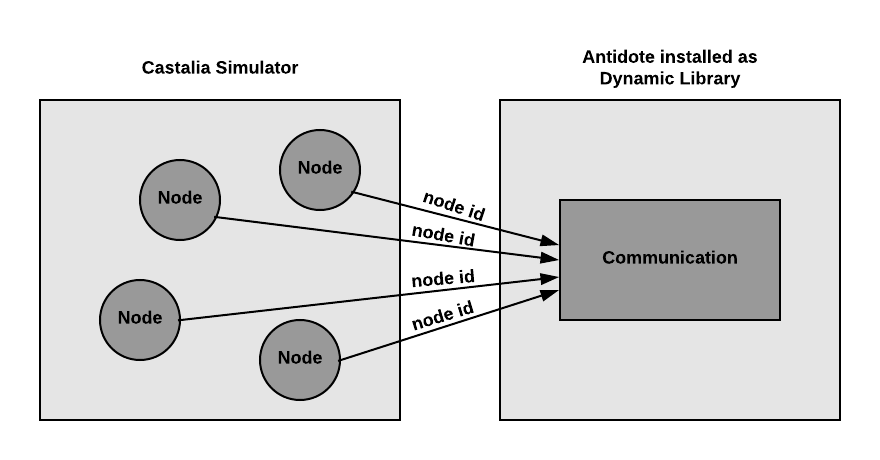
\includegraphics[scale=0.7]{figures/communicationModuleCastalia.png}}
\caption{Communication module handling several nodes}
\label{fig:communicationModuleCastalia}
\end{figure}
\section{Castalia Application Layer}

We create a application to the Castalia Application Layer. This application is agent-initiated, that is, the agent takes the initiative to send readings to the manager. The agents is the first and the only to send the association request to start sending measurements and the association release when there is no more measurements to be sent.

The current code has five agents implemented, a pulse oximeter, glucose meter, thermometer, blood pressure, and a basic ECG. The pulse oximeter transmit data like the pulse rate in beats per second and the Percentage of arterial haemoglobin oxygen saturation (SpO$_2$). The glucose meter convey the glucose level, that is, the concentration of blood sugar in the blood in milligrams per deciliter (mg\//dL) and the thermometer the temperature is in Celsius degree (\textdegree C). The blood pressure sends a data compound of systolic, diastolic and the mean arterial pressure in millimeters of mercury (mmHg). The basic ECG sends eighty samples values in each packet, each value is a millivolt (mV) sample. In the basic ECG, the seconds spacing between the samples is sent in the configuration phase as well as the lower and upper absolute value and the lower and upper scaled value. All this values are randomly produced except for basic ECG that transmit real values obtained from the data base \cite{b2}. 

The 11073 standard define confirmed and unconfirmed events. The confirmed events are message that expected an acknowledgment and the unconfirmed events doesn't expect a confirmation. Messages like \textit{Association request} and \textit{Association release} always has acknowledgments but measurements messages can be confirmed or unconfirmed. %The implemented parameter to set the desired mode is \textit{SN.node\[node number\].Application.confirmed\_event} which require a Boolean value.

\subsection{Unconfirmed measurement event}\label{sec:UnconfirmedMeasurementEvent}

Fig.\ref{fig:unconfirmedMode} shows a sequence diagram of the messaging procedure corresponding to a ordinary operation of an agent with standard configuration. The agent intends to associate with the manager for the first time and sends a \textit{Association request}. When the manager receives the \textit{Association request} it checks if there was some association made before. If not it sends an \textit{Get attributes} message along with the \textit{Association response}. So the agent sends its configuration and start to convey the measurements to the manager. When there is no more readings to transmit the agent sends a \textit{Association release} and the manager responds with an \textit{Association release response}.

\begin{figure}[htbp]
\centerline{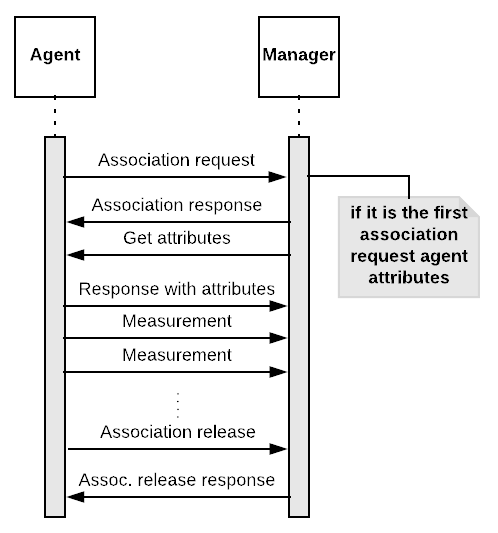
\includegraphics[scale=0.35]{figures/unconfirmed.png}}
\caption{Sequence diagram of unconfirmed operation mode of an 11073 PHD application.}
\label{fig:unconfirmedMode}
\end{figure}

\subsection{Confirmed measurement event}

\begin{figure}[htbp]
\centerline{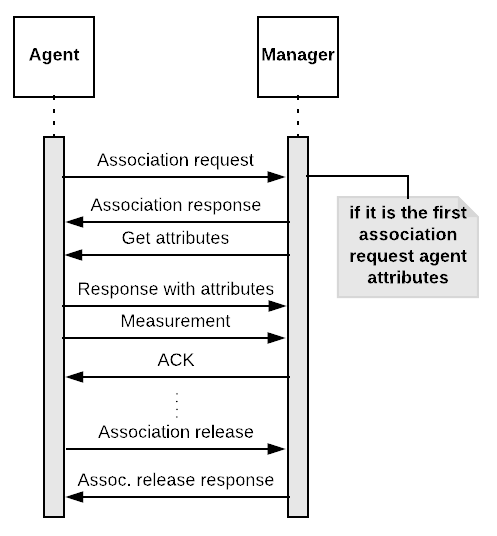
\includegraphics[scale=0.35]{figures/confirmed.png}}
\caption{Sequence diagram of confirmed operation mode of an 11073 PHD application.}
\label{fig:confirmedMode}
\end{figure}

Now the Fig.\ref{fig:confirmedMode} depicts a sequence diagram of the messaging procedure corresponding to an operation of an agent with standard configuration and with confirmed measurements events. The initial procedure is the same as explained at Section \ref{sec:UnconfirmedMeasurementEvent}. The difference is that the manager sends an acknowledgment for every measurement received. After sending a measurement data the agent shall wait three seconds. If an answer is not received in this period the agent shall send an \textit{Association abort} to the manager and transition back to the unassociated state. If the agent still has readings to send a new association must be done. This and others errors conditions is explained in \cite{b1}.

\subsection{Proposed modification in confirmed measurement event}

The 11073 standard assumes that there will be a transport layer on real devices. In the Castalia simulator as in other wireless sensor networks we do not have a transport layer, so a stop-and-wait system was implemented at the application layer for retransmission of packets that did not receive a confirmation ACK. This modification avoid many associations right after a non-received ACK.

%To avoid many associations right after a non-received ACK we implemented a stop-and-wait retransmission system in the application layer. 
This save the unnecessary exchange of several control packets. Rather than making a new association we just retransmit the packet $n$ times or until an ACK from manger is received.
%The user can define whether to retransmit and how many retransmission attempts wish.
If an ACK from the manager is lost, the agent will try to retransmit the packet $n$ times as defined by the user. When the manager finally receives the packet, it will retransmit immediately the lost ACK to the agent.

Will be shown in Results Section how this system can save many control packets exchanged when a ACK is not received. Note that this is an independent modification, not present in the 11073 standard. 
%The parameters implemented for retransmission are \textit{SN.node[nodeNumber].Application.retransmissionPacket} which require a boolean value and \textit{SN.node[nodeNumber].Application.maxNumOfRetransmition} that accepts an integer number.
\section{Results}
Using some \textit{api} from Castalia Simulator some results like the total number of control packets exchanged, the total number of measurements packets, how many times a packets was retransmited among many others results can be obtained easily.

\subsection{Use case and simulation parameters}

Monitoring and Independent living for elder care is one of the use context of 11073 standard. The sensors and devices used for this use case is described in \cite{b3} is blood pressure, thermometer, glucose meter, pulse oximeter and basic ECG. In this work we used a hypothetical elderly patient who has cardiac problems, diabetes and hypertension and  after a major surgery needs to be monitored in his home.

The Fig.~\ref{fig:wbantopology} shows the topology setup used in our simulation. The hub node is placed at the right hip, one sensor node at the right and left wrist, one sensor node at the right and left ankle and one sensor on chest. The deployment of nodes is not the ideal, we just use this set to test our feature. The positions of nodes was maintained as they are in Castalia because real experimental measurements of path loss was made for every pair of nodes in \cite{b4}.

\begin{figure}[htbp]
\centerline{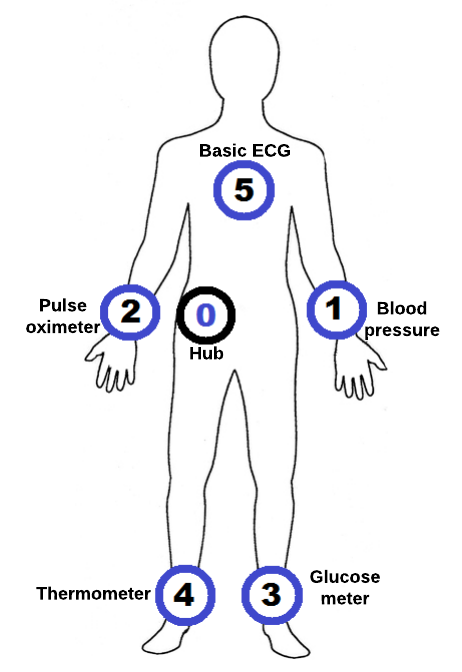
\includegraphics[scale=0.31]{figures/corpoSensoresNomes.png}}
\caption{The simulated network topology.}
\label{fig:wbantopology}
\end{figure}

In this paper we will simulate two scenario. The first scenario the agents will send measurement with no confirmation and the second with confirmation from the manager. The MAC layer used is the IEEE 802.15.6 with path loss map and temporal model for wireless channel supplied by Castalia and 1024 Kbps of physical data rate. The radio used meets with the IEEE 802.15.6 radio proposal \cite{5} and -15dBm as transmission power.

The node 0 uses the \textit{Manager} application and is the hub. The blood pressure and the pulse oximeter transmit one measurement per second. The thermometer convey one read every 2 seconds. The glucose meter  transmit one measurement every twenty five seconds. In this work we assume the basic ECG is a device that receives the signals of all electrodes deployed in the body and transmit these signals to the Manager.  
\section{Conclusion}\label{conclusion}
In this paper we presented an application to simulate personal health devices in Castalia Simulator. Our application follows the X73-PHD standard with the aid of the Antidote Library. Five agents was implemented and they simulate a real device. The users can feel free to insert more agents. As future work, we intend to develop a manager-initiated transmission where the user can set in manager the amount of meausrements to be sent.
%\section{Introduction}
% This document is a model and instructions for \LaTeX.
% Please observe the conference page limits. 

%\section{Ease of Use}

%\subsection{Maintaining the Integrity of the Specifications}

% The IEEEtran class file is used to format your paper and style the text. All margins, 
% column widths, line spaces, and text fonts are prescribed; please do not 
% alter them. You may note peculiarities. For example, the head margin
% measures proportionately more than is customary. This measurement 
% and others are deliberate, using specifications that anticipate your paper 
% as one part of the entire proceedings, and not as an independent document. 
% Please do not revise any of the current designations.

%\section{Prepare Your Paper Before Styling}
% Before you begin to format your paper, first write and save the content as a 
% separate text file. Complete all content and organizational editing before 
% formatting. Please note sections \ref{AA}--\ref{SCM} below for more information on 
% proofreading, spelling and grammar.

% Keep your text and graphic files separate until after the text has been 
% formatted and styled. Do not number text heads---{\LaTeX} will do that 
% for you.

%\subsection{Abbreviations and Acronyms}\label{AA}
% Define abbreviations and acronyms the first time they are used in the text, 
% even after they have been defined in the abstract. Abbreviations such as 
% IEEE, SI, MKS, CGS, ac, dc, and rms do not have to be defined. Do not use 
% abbreviations in the title or heads unless they are unavoidable.

%\subsection{Units}
% \begin{itemize}
% \item Use either SI (MKS) or CGS as primary units. (SI units are encouraged.) English units may be used as secondary units (in parentheses). An exception would be the use of English units as identifiers in trade, such as ``3.5-inch disk drive''.
% \item Avoid combining SI and CGS units, such as current in amperes and magnetic field in oersteds. This often leads to confusion because equations do not balance dimensionally. If you must use mixed units, clearly state the units for each quantity that you use in an equation.
% \item Do not mix complete spellings and abbreviations of units: ``Wb/m\textsuperscript{2}'' or ``webers per square meter'', not ``webers/m\textsuperscript{2}''. Spell out units when they appear in text: ``. . . a few henries'', not ``. . . a few H''.
% \item Use a zero before decimal points: ``0.25'', not ``.25''. Use ``cm\textsuperscript{3}'', not ``cc''.)
% \end{itemize}

%\subsection{Equations}
% Number equations consecutively. To make your 
% equations more compact, you may use the solidus (~/~), the exp function, or 
% appropriate exponents. Italicize Roman symbols for quantities and variables, 
% but not Greek symbols. Use a long dash rather than a hyphen for a minus 
% sign. Punctuate equations with commas or periods when they are part of a 
% sentence, as in:
% \begin{equation}
% a+b=\gamma\label{eq}
% \end{equation}

% Be sure that the 
% symbols in your equation have been defined before or immediately following 
% the equation. Use ``\eqref{eq}'', not ``Eq.~\eqref{eq}'' or ``equation \eqref{eq}'', except at 
% the beginning of a sentence: ``Equation \eqref{eq} is . . .''

%\subsection{\LaTeX-Specific Advice}

% Please use ``soft'' (e.g., \verb|\eqref{Eq}|) cross references instead
% of ``hard'' references (e.g., \verb|(1)|). That will make it possible
% to combine sections, add equations, or change the order of figures or
% citations without having to go through the file line by line.

% Please don't use the \verb|{eqnarray}| equation environment. Use
% \verb|{align}| or \verb|{IEEEeqnarray}| instead. The \verb|{eqnarray}|
% environment leaves unsightly spaces around relation symbols.

% Please note that the \verb|{subequations}| environment in {\LaTeX}
% will increment the main equation counter even when there are no
% equation numbers displayed. If you forget that, you might write an
% article in which the equation numbers skip from (17) to (20), causing
% the copy editors to wonder if you've discovered a new method of
% counting.

% {\BibTeX} does not work by magic. It doesn't get the bibliographic
% data from thin air but from .bib files. If you use {\BibTeX} to produce a
% bibliography you must send the .bib files. 

% {\LaTeX} can't read your mind. If you assign the same label to a
% subsubsection and a table, you might find that Table I has been cross
% referenced as Table IV-B3. 

% {\LaTeX} does not have precognitive abilities. If you put a
% \verb|\label| command before the command that updates the counter it's
% supposed to be using, the label will pick up the last counter to be
% cross referenced instead. In particular, a \verb|\label| command
% should not go before the caption of a figure or a table.

% Do not use \verb|\nonumber| inside the \verb|{array}| environment. It
% will not stop equation numbers inside \verb|{array}| (there won't be
% any anyway) and it might stop a wanted equation number in the
% surrounding equation.

%\subsection{Some Common Mistakes}\label{SCM}
% \begin{itemize}
% \item The word ``data'' is plural, not singular.
% \item The subscript for the permeability of vacuum $\mu_{0}$, and other common scientific constants, is zero with subscript formatting, not a lowercase letter ``o''.
% \item In American English, commas, semicolons, periods, question and exclamation marks are located within quotation marks only when a complete thought or name is cited, such as a title or full quotation. When quotation marks are used, instead of a bold or italic typeface, to highlight a word or phrase, punctuation should appear outside of the quotation marks. A parenthetical phrase or statement at the end of a sentence is punctuated outside of the closing parenthesis (like this). (A parenthetical sentence is punctuated within the parentheses.)
% \item A graph within a graph is an ``inset'', not an ``insert''. The word alternatively is preferred to the word ``alternately'' (unless you really mean something that alternates).
% \item Do not use the word ``essentially'' to mean ``approximately'' or ``effectively''.
% \item In your paper title, if the words ``that uses'' can accurately replace the word ``using'', capitalize the ``u''; if not, keep using lower-cased.
% \item Be aware of the different meanings of the homophones ``affect'' and ``effect'', ``complement'' and ``compliment'', ``discreet'' and ``discrete'', ``principal'' and ``principle''.
% \item Do not confuse ``imply'' and ``infer''.
% \item The prefix ``non'' is not a word; it should be joined to the word it modifies, usually without a hyphen.
% \item There is no period after the ``et'' in the Latin abbreviation ``et al.''.
% \item The abbreviation ``i.e.'' means ``that is'', and the abbreviation ``e.g.'' means ``for example''.
% \end{itemize}
% An excellent style manual for science writers is \cite{b7}.

%\subsection{Authors and Affiliations}
% \textbf{The class file is designed for, but not limited to, six authors.} A 
% minimum of one author is required for all conference articles. Author names 
% should be listed starting from left to right and then moving down to the 
% next line. This is the author sequence that will be used in future citations 
% and by indexing services. Names should not be listed in columns nor group by 
% affiliation. Please keep your affiliations as succinct as possible (for 
% example, do not differentiate among departments of the same organization).

%\subsection{Identify the Headings}
% Headings, or heads, are organizational devices that guide the reader through 
% your paper. There are two types: component heads and text heads.

% Component heads identify the different components of your paper and are not 
% topically subordinate to each other. Examples include Acknowledgments and 
% References and, for these, the correct style to use is ``Heading 5''. Use 
% ``figure caption'' for your Figure captions, and ``table head'' for your 
% table title. Run-in heads, such as ``Abstract'', will require you to apply a 
% style (in this case, italic) in addition to the style provided by the drop 
% down menu to differentiate the head from the text.

% Text heads organize the topics on a relational, hierarchical basis. For 
% example, the paper title is the primary text head because all subsequent 
% material relates and elaborates on this one topic. If there are two or more 
% sub-topics, the next level head (uppercase Roman numerals) should be used 
% and, conversely, if there are not at least two sub-topics, then no subheads 
% should be introduced.

%\subsection{Figures and Tables}
% \paragraph{Positioning Figures and Tables} Place figures and tables at the top and 
% bottom of columns. Avoid placing them in the middle of columns. Large 
% figures and tables may span across both columns. Figure captions should be 
% below the figures; table heads should appear above the tables. Insert 
% figures and tables after they are cited in the text. Use the abbreviation 
%``Fig.~\ref{fig}'', even at the beginning of a sentence.

% \begin{table}[htbp]
% \caption{Table Type Styles}
% \begin{center}
% \begin{tabular}{|c|c|c|c|}
% \hline
% \textbf{Table}&\multicolumn{3}{|c|}{\textbf{Table Column Head}} \\
% \cline{2-4} 
% \textbf{Head} & \textbf{\textit{Table column subhead}}& \textbf{\textit{Subhead}}& \textbf{\textit{Subhead}} \\
% \hline
% copy& More table copy$^{\mathrm{a}}$& &  \\
% \hline
% \multicolumn{4}{l}{$^{\mathrm{a}}$Sample of a Table footnote.}
% \end{tabular}
% \label{tab1}
% \end{center}
% \end{table}

% \begin{figure}[htbp]
% \centerline{\includegraphics{fig1.png}}
% \caption{Example of a figure caption.}
% \label{fig}
% \end{figure}

% Figure Labels: Use 8 point Times New Roman for Figure labels. Use words 
% rather than symbols or abbreviations when writing Figure axis labels to 
% avoid confusing the reader. As an example, write the quantity 
% ``Magnetization'', or ``Magnetization, M'', not just ``M''. If including 
% units in the label, present them within parentheses. Do not label axes only 
% with units. In the example, write ``Magnetization (A/m)'' or ``Magnetization 
% \{A[m(1)]\}'', not just ``A/m''. Do not label axes with a ratio of 
% quantities and units. For example, write ``Temperature (K)'', not 
% ``Temperature/K''.

%\section*{Acknowledgment}

% The preferred spelling of the word ``acknowledgment'' in America is without 
% an ``e'' after the ``g''. Avoid the stilted expression ``one of us (R. B. 
% G.) thanks $\ldots$''. Instead, try ``R. B. G. thanks$\ldots$''. Put sponsor 
% acknowledgments in the unnumbered footnote on the first page.

%\section*{References}

% Please number citations consecutively within brackets \cite{b1}. The 
% sentence punctuation follows the bracket \cite{b2}. Refer simply to the reference 
% number, as in \cite{b3}---do not use ``Ref. \cite{b3}'' or ``reference \cite{b3}'' except at 
% the beginning of a sentence: ``Reference \cite{b3} was the first $\ldots$''

% Number footnotes separately in superscripts. Place the actual footnote at 
% the bottom of the column in which it was cited. Do not put footnotes in the 
% abstract or reference list. Use letters for table footnotes.

% Unless there are six authors or more give all authors' names; do not use 
% ``et al.''. Papers that have not been published, even if they have been 
% submitted for publication, should be cited as ``unpublished'' \cite{b4}. Papers 
% that have been accepted for publication should be cited as ``in press'' \cite{b5}. 
% Capitalize only the first word in a paper title, except for proper nouns and 
% element symbols.

% For papers published in translation journals, please give the English 
% citation first, followed by the original foreign-language citation \cite{b6}.

% \vspace{12pt}
% \color{red}
% IEEE conference templates contain guidance text for composing and formatting conference papers. Please ensure that all template text is removed from your conference paper prior to submission to the conference. Failure to remove the template text from your paper may result in your paper not being published.

\begin{thebibliography}{00}
% \bibitem{b1} G. Eason, B. Noble, and I. N. Sneddon, ``On certain integrals of Lipschitz-Hankel type involving products of Bessel functions,'' Phil. Trans. Roy. Soc. London, vol. A247, pp. 529--551, April 1955.
\bibitem{b1} Health informatics - Personal health device communication, Part 20601: Application profile - Optimized exchange protocol, 2016.

%\bibitem{b2} J. Clerk Maxwell, A Treatise on Electricity and Magnetism, 3rd ed., vol. 2. Oxford: Clarendon, 1892, pp.68--73.
\bibitem{b2} Goldberger AL, Amaral LAN, Glass L, Hausdorff JM, Ivanov PCh, Mark RG, Mietus JE, Moody GB, Peng CK, Stanley HE. PhysioBank, PhysioToolkit, and PhysioNet: Components of a New Research Resource for Complex Physiologic Signals. Circulation 101(23):e215-e220 Circulation Electronic Pages; \url{http://circ.ahajournals.org/content/101/23/e215.full}; 2000 (June 13). PMID: 10851218; doi: 10.1161 01.CIR.101.23.e215.

%\bibitem{b3} I. S. Jacobs and C. P. Bean, ``Fine particles, thin films and exchange anisotropy,'' in Magnetism, vol. III, G. T. Rado and H. Suhl, Eds. New York: Academic, 1963, pp. 271--350.
\bibitem{b3}  Health Informatics - Personal health device communication Part 00103: Overview, 2012.

%\bibitem{b4} K. Elissa, ``Title of paper if known,'' unpublished.
\bibitem{b4} Boulis, A., Tselishchev, Y. (2010). Contention vs. polling: A study in body area networks MAC design. Proceedings of the Fifth International Conference on Body Area Networks, 98–104. \url{https://doi.org/10.1145/2221924.2221944}

%\bibitem{b5} R. Nicole, ``Title of paper with only first word capitalized,'' J. Name Stand. Abbrev., in press.
\bibitem{b5} IEEE Std 802.15.6-2012, IEEE Standard for Local and metropolitan area networks - Part 15.6: Wireless Body Area Networks, no. February. 2012.

%\bibitem{b6} Y. Yorozu, M. Hirano, K. Oka, and Y. Tagawa, ``Electron spectroscopy studies on magneto-optical media and plastic substrate interface,'' IEEE Transl. J. Magn. Japan, vol. 2, pp. 740--741, August 1987 [Digests 9th Annual Conf. Magnetics Japan, p. 301, 1982].
\bibitem{b6} Benedetti, D., Petrioli, C., Spenza, D. (2013). GreenCastalia: An Energy-Harvesting-Enabled Framework for the Castalia Simulator. Proceedings of the 1st International Workshop on Energy Neutral Sensing Systems - ENSSys ’13, 1–6. \url{https://doi.org/10.1145/2534208.2534215}

%\bibitem{b7} M. Young, The Technical Writer's Handbook. Mill Valley, CA: University Science, 1989.
\bibitem{b7}
Martins, A. F., Santos, D. F. S., Perkusich, A., Almeida, H. O. (2014). IEEE 11073 and connected health: Preparing personal health devices for the Internet. Digest of Technical Papers - IEEE International Conference on Consumer Electronics, 274–275. \url{https://doi.org/10.1109/ICCE.2014.6776001}

\bibitem{b8} Gomes, Y. F., Santos, D. F. S., Almeida, H. O., Perkusich, A. (2015). Integrating MQTT and ISO / IEEE 11073 for Health Information Sharing in the Internet of Things. 2015 IEEE International Conference on Consumer Electronics (ICCE), 200–201.

\bibitem{b9} Santos, D. F. S., Bublitz, F. M., Almeida, H. O., Perkusich, A. (2014). Integrating IEEE 11073 and constrained application protocol for personal health devices. Proceedings of the 29th Annual ACM Symposium on Applied Computing - SAC ’14, (March), 466–467. \url{https://doi.org/10.1145/2554850.2555145}

\bibitem{b10} Santos, D. F. S., Almeida, H. O., Perkusich, A. (2015). A personal connected health system for the Internet of Things based on the Constrained Application Protocol. Computers and Electrical Engineering, 44, 122–136. \url{https://doi.org/10.1016/j.compeleceng.2015.02.020}

\bibitem{b11} Clarke, M., De Folter, J., Verma, V., Gokalp, H. (2018). Interoperable End-to-End Remote Patient Monitoring Platform Based on IEEE 11073 PHD and ZigBee Health Care Profile. IEEE Transactions on Biomedical Engineering, 65(5), 1014–1025. \url{https://doi.org/10.1109/TBME.2017.2732501}

\bibitem{b12} International, H. (2019). Health Level Seven International - Homepage | HL7 International. [online] Hl7.org. Available at: \url{http://www.hl7.org/index.cfm} [Accessed 7 Jan. 2019].

\bibitem{b13} IHE International. (2019). Integrating the Healthcare Enterprise (IHE) - IHE International. [online] Available at: \url{https://www.ihe.net/} [Accessed 7 Jan. 2019].

\bibitem{b14} Barrón-González, H. G., Martínez-Espronceda, M., Trigo, J. D., Led, S., Serrano, L. (2016). Lessons learned from the implementation of remote control for the interoperability standard ISO/IEEE11073-20601 in a standard weighing scale. Computer Methods and Programs in Biomedicine, 123, 81–93. \url{https://doi.org/10.1016/j.cmpb.2015.09.015}

\bibitem{b15} Boulis, Athanassios. Castalia: A simulator for Wireless Sensor Networks and Body Area Networks (User's manual). Version 3.3, NICTA. May 2013. [online] Available at: \url{https://github.com/boulis/Castalia} [Accessed 7 Jan. 2019].

\bibitem{b16} IEEE Std 11073-20101 (2004). Health informatics-point-of-care medical
device communication - part 20101: Application profile-base standard. Standard, ISO/IEEE, New York, USA.

\bibitem{b17} Benner, M., Schöpe, L. (2011). Using continua health alliance standards: Implementation and experiences of IEEE 11073. Proceedings - IEEE International Conference on Mobile Data Management, 2, 40–45. \url{https://doi.org/10.1109/MDM.2011.25}

\end{thebibliography}

\end{document}
